\documentclass{article}[18pt]
\usepackage{../../../../format}
\lhead{Software Methodologies - Machine Learning}


\begin{document}
\begin{center}
\underline{\Large Cost Function, Binary Classifier and Performance Measurement}
\end{center}
\section{Cost Functions}
Supervised learning problem
\begin{itemize}
	\item Collection of n p-dimensional feature vectors: \hfill $\{x_i\}, i=1...n$
	\item Collection of observed responses \hfill $\{y_i\},i=1...n$
	\item Aims to construct a response surface \hfill $h(x)$
\end{itemize}
\begin{itemize}
	\item Describes how well the current response surface $h(x)$ fits the available data (on a given set) - we use J to represent the cost function
	$$J(y_i,h(x_i))$$
	\item Smaller values of the cost function correspond to a better fit, so in the graph below $J_2>J_1$
	\item Machine learning goal: construct $h(x)$ such that J is minimised
	\item In regression, $h(x)$ is usually directly interpretable as a predicted response
\end{itemize}
\begin{center}
	\includegraphics[scale=0.7]{"Cost Function"}
\end{center}
\subsection{Least squares deviation cost}
$$J(y_i,h(x_i))=\dfrac{1}{n}\sum_{i=1}^{n}{(y_i-h(x_i))^2}$$
$r_i$ is the difference between the real value and the predicted value 
\begin{itemize}
	\item Nice mathematical properties
	\item Problem with outliers- when you have a large residual and it is then squared, the impact is large where it should be ignored
\end{itemize}

\begin{center}
	\includegraphics[scale=0.7]{"Least Squares Deviation"}
\end{center}
\subsection{Least Absolute Deviation Cost}
$$J(y_i,h(x_i))=\dfrac{1}{n}\sum_{i=1}^{n}{|(y_i-h(x_i))|}$$
\begin{itemize}
	\item More robust with respect to outliers - not squared residual so less impact
	\item May pose computational challenges
\end{itemize}
\begin{center}
	\includegraphics[scale=0.7]{"Least Absolute Deviation"}
\end{center}
\subsection{Huber-M Cost}
$$J(y_i,h(x_i))=\dfrac{1}{n}\sum_{i=1}^{n}\left\{\begin{array}{lr}
0.5(y_i-h(x_i))^2 & \text{if } |y_i-h(x_i)|<\delta\\
\delta({|y_i-h(x_i)|}-0.5\delta) & \text{otherwise}\\
\end{array}\right\}$$
\begin{itemize}
	\item Combines the best qualities of the LS and LAD losses (basically using one or the other depending on which one is better to use)
	\item Parameter $\delta$ is usually set automatically to a specific percentile of absolute residuals. Calculate all residuals, then for example top 10\% is $\delta$
\end{itemize}
\begin{center}
	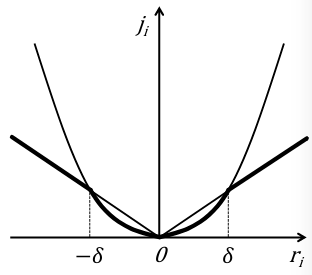
\includegraphics[scale=0.7]{Huber-M}
\end{center}
\newpage
\section{Binary Classifier}
\begin{itemize}
	\item Observed response y takes only two possible values + and -
	\item Define relationship between $h(x)$ and $y$
	\item If larger than the threshold, then set to 1, if less then set to 0
	\item Use the decision rule:
	\[
	\hat{y}=\left\{\begin{array}{ll}
	{+,} & {h(x) \geq t} \\
	{-,} & {\text { otherwise }}
	\end{array}\right.
	\]
\end{itemize}
\begin{center}
	\includegraphics[scale=0.7]{"Binary Classifier"}
\end{center}
\section{Performance Measures}
\subsection{Precision and Recall}
How well did we capture the + group for the given threshold
\begin{center}
	\includegraphics[scale=0.7]{"Precision and Recall"}
\end{center}
\begin{center}
	\includegraphics[scale=0.7]{"Precision and Recall1"}
\end{center}
Precision:
$$\dfrac{tp}{tp+fp}>1$$
Recall (Sensitivity)
$$\dfrac{tp}{tp+fn}>1$$
\begin{center}
	\includegraphics[scale=0.7]{"Precision and Recall2"}
\end{center}
\subsection{ROC Curve}
Recall (sensitivity)
$$\dfrac{tp}{tp+fn}$$
Specificity
$$\dfrac{tn}{tn+fp}$$
\begin{center}
	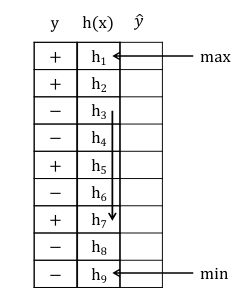
\includegraphics[scale=0.7]{ROC}
\end{center}
\begin{center}
	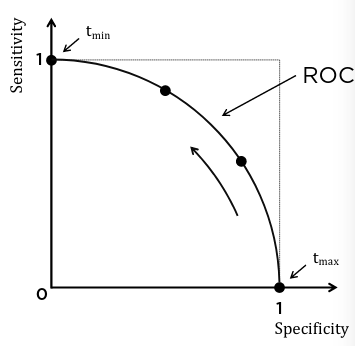
\includegraphics[scale=0.7]{ROC1}
\end{center}
\subsection{Gains and Lift}
Sensitivity (recall)
$$Se=\dfrac{tp}{tp+fn}$$
Support (\% pop)
$$Su=\dfrac{tp+fp}{n}$$
\begin{center}
	\includegraphics[scale=0.7]{"Gains and Lift"}
\end{center}
Base rate
$$Br=\dfrac{tp+fn}{n}$$
Gains
$$\{Su,Se\}$$
Lift
$$\{Su,\dfrac{Se}{Su}\}$$
ROC
$$\{\dfrac{Su-Br\cdot Se}{1-Br},Se\}$$














\end{document}